\chapter{Anwendung}
Dieses Kapitel soll die Interessantesten Teile der Anwendung Dokumentieren. Mit dem Vorangegangen Code lassen sich alle nicht dokumentierte Teile im Code sehr gut nachvollziehen.



\section{Anlegen, Aktualisieren, Löschen und Ausgeben von Gegenständen}
Im Frontend werden neue Gegenstände über ein Formular gesendet. Die Inhalte des Formulars werden per \ac{JSON} mittels POST an die Restschnittstelle von Laravel gesendet, welche der Controller verarbeitet und in die Datenbank einträgt. Sollte ein Barcode schon vorhanden sein, wird der User darauf hingewiesen. Bei einer Löschung, Aktualisierung oder einer Ausgabe muss nur darauf hingewiesen werden, um welches Item es sich genau handelt.

\begin{lstlisting}[language=php, frame=single]
public function postItem(Request $request)
{
$item = new Item();
$item->barcode = $request->input('barcode');
$item->name = $request->input('name');
$item->description = $request->input('description');
$item->type = $request->input('type');
$item->room = $request->input('room');
$item->status = $request->input('status');
$item->annotation = $request->input('annotation');
$item->image = $request->input('image');
$item->lend = $request->input('lend');
$item->manufactor = $request->input('manufactor');
$item->save();
return response()->json($item, 201);

}

public function getItems(){
$items = Item::all();
$response = [
'items' => $items
];
return response()->json($response,200);
}

public function putItem(Request $request, $id){
$item = Item::find($id);
if(!$item){
return response()->json(['message'=>'Document not found Barcode: '. $id . '. The number is not the Barcode. Look into the Table'], 400);

}
$item->name = $request->input('name');
$item->description = $request->input('description');
$item->type = $request->input('type');
$item->room = $request->input('room');
$item->status = $request->input('status');
$item->annotation = $request->input('annotation');
$item->image = $request->input('image');
$item->lend = $request->input('lend');
$item->manufactor = $request->input('manufactor');
$item->save();
return response()->json(['item' => $item], 200);
}

public function putItemLendBack( $id){
$item = Item::find($id);
if(!$item){
return response()->json(['message'=>'Document not found putItemLendBack: '. $id . '. The number is not the Barcode. Look into the Table'], 400);

}

$item->status = 'back';

$item->save();
return response()->json(['item' => $item], 200);
}

public function deleteItem($id){
$item = Item::find($id);
$item->delete();
return response()->json(['message' => 'Deleted'],200);

}

public function getItem($id){
$item = Item::find($id);
if(!$item){
return response()->json(['message'=>'Document not found ID: '. $id . '. The number is not the Barcode. Look into the Table'], 400);

}

$response = [
'items' => $item
];

return response()->json($response,200);


}
\end{lstlisting}

\begin{figure}[H]
	\centering
	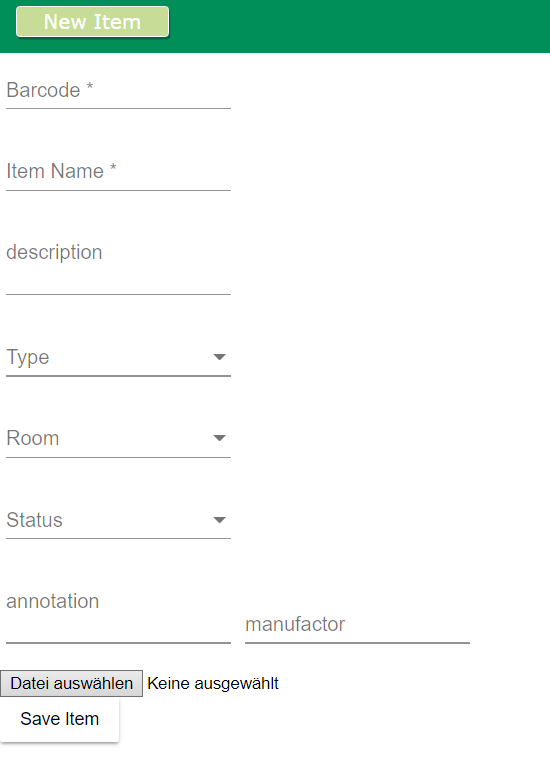
\includegraphics[scale=0.5]{content/pictures/item.png}
	% bosch_iot_poll.png: 0x0 pixel, 300dpi, 0.00x0.00 cm, bb=
	\caption{Anlegen von Items}
	\label{fig:item}
\end{figure}

\section{Ausgabe von allen Gegenständen}
Um eine Liste aller Gegenstände wird vom Server eine \ac{JSON} generiert, welche mit in Angular in einer Tabelle ausgegeben werden. Hierfür wurde Angular Material verwendet, welches die Tabelle auch gleichzeitig gestaltet hat.

\begin{lstlisting}[language=html, frame=single]
<mat-table [dataSource]='dataSource' matSort>

<ng-container matColumnDef="barcode">
<mat-header-cell *matHeaderCellDef mat-sort-header>Barcode</mat-header-cell>
<mat-cell *matCellDef="let items">{{items.barcode}}</mat-cell>
</ng-container>

.
.
.

<mat-header-row *matHeaderRowDef="displayedColumns"></mat-header-row>
<mat-row *matRowDef="let row; columns: displayedColumns;"></mat-row>

</mat-table>
\end{lstlisting}


\section{Routing Strategie}
Wie in Kapitel \ref{webauftritt} beschrieben, wird der Webauftritt von WordPress verwaltet. WordPress selbst nutzt das Routing um Verschiedene Seiten anzeigen zu können. Läuft eine Angular Anwendung auf dem gleichen Server, oder soll sie gar in WordPress eingebunden werden, kann das zu Problemen führen, da sie die gleiche Strategie nutzen. Eine Unterseite in Angular aufzurufen ist nicht möglich wenn man es zuvor nicht konfiguriert. WordPress wird immer eine Fehlerseite werfen, sofern nicht eine Unterseite von WordPress den gleichen Namen trägt. Aber auch in diesem Fall wird eine Falsche Seite dem User Präsentiert.

Eine Lösung ist die \textit{HashLocationStrategy}. Bei dieser Strategie muss der Anwendung mit einem Konfigurationsbefehl mitgeteilt werden, wie das Routing ab sofort funktionieren soll. Dabei wird vor der dem eigentlich Anhängen der Unterseite ein Rautensymbol angehangen. Damit kann Wordpress in der Regel nur die Startseite Anzeigen und wird nicht auf eine Fehlerhafte Seite verweisen. Somit ist ein Routing unter der gleichen Domain möglich und es ist trotz allem für den User nachvollziehbar. 

\begin{lstlisting}[language=sh, frame=single]
RouterModule.forRoot(routes, {useHash: true})
\end{lstlisting}

Es ist nur useHash im Routermodul auf true zusetzen und Angular erledigt den rest. Die variable routes ist ein Array, welches alle Routen verwaltet.



\section{E-Mail Reminder}
Für den Reminder (\ac{z. Dt.} Erinnerer) wird eine Konfiguration angelegt, in welcher definiert wird was in der E-Mail stehen soll, welche der User erhalten wird. Dabei handelt es sich um ein Template. Alle nötigen Daten holt sich Laravel selbständig aus der Datenbank. Ein Anlegen eines solchen Schedulars wird im folgenden Code Beispiel Demonstriert.
\begin{lstlisting}[language=php, frame=single]
protected function schedule(Schedule $schedule)
{
		$schedule->command('reminder:mail')->daily();
}
\end{lstlisting}

\section{Datenbank import und export}
Für einen unerfahrenen User soll es leicht sein Daten zu importieren und für eine Sicherung oder zur Nutzung ohne Netzwerkverbindung zu nutzen. Auch kann es sein, das viele Daten Angelegt werden sollen, welche einfacher oder schneller über eine Tabelle angelegt werden könnten. Dabei soll der User keine Daten anlegen oder mit Programmen arbeiten müssen, welche ihm unbekannt sind. Eine sehr Bekannte Möglichkeit solche Dateien zu erstellen ist Microsoft Excel. Der User soll eine Excel-Datei erstellen und diese über ein grafische Benutzeroberfläche importieren können. Dabei darf es keine Rolle spielen welche Endung die Excel-Datei hat. Mit einem Export soll ebenfalls eine Excel-Datei erzeugt werden.

Für den Import wurde mittels Composer die Erweiterung PHPOffice verwendet. Es kann Excel-Dateien lesen und schreiben. Mit dem Lesen werden die Daten in die Datenbank geschrieben. Hierbei wird Dopplung vermieden und wenn es sich um bekannte deutsche Begriffe handelt, werden diese auf englisch in die Datenbank geschrieben. Sollte ein Begriff unbekannt sein, so wird der deutsche Wortlaut übernommen. Um Dopplung zu vermeiden musste ein eindeutiger Schlüssel gewählt werden. Die Entscheidung fiel auf den Barcode. Hat ein neu angelegtes Item keinen Barcode, wird es nicht importiert. Dieser ist zwingend nötig. Der Export wird ebenfalls von PHPOffice übernommen. Hierbei muss nur Angegeben werden, wie jede Spalte heißt. Der User kann nun sich einmalig eine Tabelle Exportieren lassen und diese nach diesem Schema füllen und Importieren. Die Exportieren Funktion findet der User Unter dem Button Backup.

\begin{lstlisting}[language=php, frame=single]
public function insertItemsInDatabase()
{
	$inputFileName = public_path() . '\table\barcode.xlsx';
	$inputFileType = IOFactory::identify($inputFileName);
	
	$reader = new \PhpOffice\PhpSpreadsheet\Reader\Xlsx();
	
	
	$reader->setReadFilter(new MyReadFilter());
	
	//Einlesen
	$spreadsheet = $reader->load($inputFileName);
	
	$sheetData = $spreadsheet->getActiveSheet()->toArray(null, true, true, true);
	
	
	//alle datein eintragen und übersetzen
	foreach ($sheetData as $row){
		
		$name ="";
		$barcode ="";
		$description ="";
		$room ="";
		$status ="";
		$type ="";
		$annotation ="";
		$image ="";
		$lend ="";
		$manufactor ="";
		
		
		
		//Übersetzung
		if($row['F'] == 'Zubehör'){
			$type = 'equipment';
		}
	
	...	
		
		//Abbruchkreterium
		if (DB::table('items')->where('barcode', '=', $barcode)->count() > 0) {
			continue;
			
		}
		else{
			DB::table('items')->insert(
			['barcode'=> $barcode, 'name' => $name, 'description' => $description,
			'type' => $type, 'room' => $room, 'status' => $status]
			);
		}
			
		
	}
	
	return response()->json($sheetData, 200);
	
}
\end{lstlisting}

\begin{lstlisting}[language=php, frame=single]
 public function exportItemsInXml(){
//Überschriften für die Spalten
$spreadsheet = new Spreadsheet();
$sheet = $spreadsheet->getActiveSheet();
$sheet->setCellValue('A1', 'Artikel');
$sheet->setCellValue('B1', 'Barcode');
$sheet->setCellValue('C1', 'Bezeichnung');
$sheet->setCellValue('C1', 'Bezeichnung');
$sheet->setCellValue('D1', 'Einsatzbereich');
$sheet->setCellValue('E1', 'Position');
$sheet->setCellValue('F1', 'Kategorie');
$sheet->setCellValue('G1', 'Status');

$items = Item::all();

$exportFileName = "table\\barcode_export.xlsx";

//Eintragen der Daten
foreach ($items as $item){
$sheet->setCellValue('A' . $index, $item->name);
$sheet->setCellValue('B'  . $index, $item->barcode);
$sheet->setCellValue('C' . $index, $item->description);

$sheet->setCellValue('D' . $index, $item->room);
$sheet->setCellValue('E' . $index, 'unknown');
$sheet->setCellValue('F' . $index, $item->type);
$sheet->setCellValue('G' . $index, $item->status);
$index++;
}

$writer = new Xlsx($spreadsheet);



$writer->save($exportFileName);



//in eine Datei schreiben.
return response()->download(public_path('table\\barcode_export.xlsx'))->deleteFileAfterSend();

}
\end{lstlisting}

\begin{figure}[H]
	\centering
	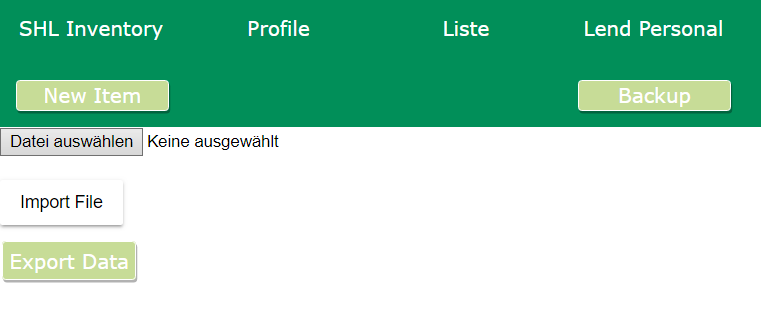
\includegraphics[scale=0.5]{content/pictures/backup.png}
	% bosch_iot_poll.png: 0x0 pixel, 300dpi, 0.00x0.00 cm, bb=
	\caption{ Importieren und Exportieren von Items}
	\label{fig:backup}
\end{figure}

\section{Gestalten der Navigationsleiste}
Die Webanwendung ist nicht responsiv. Was heiß das sich nicht auf allen Endgeräten perfekt dargestellt und nur auf einem PC oder Tablett komfortabel genutzt werden kann. Jedoch wurde mittels \ac{CSS}3 eine Navigation gestaltet, welche sich der Größe des Browsers anpasst.


\begin{lstlisting}[language=php, frame=single]
.felx-container {
	display: flex;
	background-color: #018F59;
	width: 100%;
	margin-left: auto;
	margin-right: auto;
	flex-direction: row;
	flex-wrap: wrap;
	justify-content: space-between;
	
	span {
		color: white;
		margin: .8rem;
		width: 120px;
		text-align: center;
		
		
	}
	
}

\end{lstlisting}